\documentclass[11pt, oneside]{article}   	% use "amsart" instead of "article" for AMSLaTeX format
\usepackage[a4paper]{geometry}                		% See geometry.pdf to learn the layout options. There are lots.
\geometry{letterpaper}   
%\geometry{left=2.5cm,right=2.5cm,top=2.5cm,bottom=2.5cm}                   		% ... or a4paper or a5paper or ... 
%\geometry{landscape}                		% Activate for rotated page geometry
%\usepackage[parfill]{parskip}    		% Activate to begin paragraphs with an empty line rather than an indent
\usepackage{graphicx}				% Use pdf, png, jpg, or eps§ with pdflatex; use eps in DVI mode
								% TeX will automatically convert eps --> pdf in pdflatex		
\usepackage{amssymb}
\usepackage{appendix}
\usepackage{subfigure}

%SetFonts

%SetFonts

\title{\bf A new DSL for IoT Synchronization}
\author{\sffamily FAN Qiyue\\{\sffamily\small Dept. Digital Science}\\{\sffamily\small ENSEEIHT}}
\date{}							% Activate to display a given date or no date

\begin{document}
\maketitle

{\noindent\small{\bf Abstract:} In this research, we rely on Model-Driven Engineering to propose a new DSL (Domain Specific language) for IoT. The case study applies for healthcare field, more specifically signal synchronization between both EEG and ECG devices. The main goal is to ensure the transformation from model into Java to automatically generate executable code for simulation experiments, and into formal language LOTOS in order to rigorously check needed properties.}

\vspace{1ex}
{\noindent\small{\bf Keywords:}
    IoT, MDE, Signal Synchronization, Distributed System, LOTOS.}



\section{Introduction}
\indent \par The various Internet of Things systems are gradually penetrating into all aspects of our lives and work. Here we focus on its application in the healthcare field. This field usually needs to compare the data collected by multiple sensors, and human body signals may have quite different natures, for example, the heartbeat signal can be treated as continuous signal, while the ERP signal is event-driven one. So before experts compare them together, it requires these data be strictly synchronized in time. However, different sensors have different manufacturers, operating platforms, clock accuracies, etc. Resulting in their local clocks usually unable to guarantee the synchronization. This research aims to solve the synchronization problem between multiple signals from the perspective of Model-Driven Engineering, before conducting joint analysis on them.\par
\indent \par Model-Driven Engineering approach can provide a formal verification, and also can improve reusability and scalability of the whole system. We use a case of ECG and EEG signals synchronization throughout the paper as study case.\par

\section{State of the Art}
%%\indent \par 

\indent \par IoT technologies have been widely used in healthcare domains, Machado, Sergio et al. \cite{ref2} compared the topographic distribution of cortical activation between real and imagined movement through ERP. Huang G. et al. \cite{ref3} studied the effect of window function on power density estimation of EEG signals. Covantes-Osuna C. et al. \cite{ref4} compared the different windows performance in EEG signals related to movement intention, and find the adequate window in specific frequency bands filters. The results suggested the Barlett is the suitable window to study the spectral information of the movement intention in EEG records. B. Ramachandran and S. Bashyam \cite{ref11} proposed a ECG signal monitoring system based on LabVIEW. A micro-controller obtains the input from the ECG sensors. The LabVIEW Biomedical Toolkit Package is used to convert the processed electrical impulse signal into a visual representation. The abnormality detected in heart rate is sent via SMS using the GSM module, however, it is only for this specific application, and the reusabily remains little.\par


\indent \par These systems can usually be treated as hybrid systems. Alur and Rajeev  \cite{ref8} reviewed selected existing approaches to formal verification of hybrid systems. Including symbolic reachability analysis and deductive verification. The tool HyTech was the first model checker to implement symbolic reachability analysis and the tool KeYmaera offers support to prove correctness of hybrid systems using deductive verification. A. Filieri et al. \cite{ref10} introduced a control design process for software systems. The goal is to bootstrap the design of mathematically grounded controllers, sensors, and actuators for self-adaptive software systems, providing formally provable effectiveness, efficiency and robustness. But it still needs appropriate sensors (e.g., to observe the frame rate) and actuators (e.g., to adapt the encoding quality), and a runtime with a protocol that connects these sensors and effectors with the controller, which is usually hard to achieve. \par

	
\indent \par Synchronization is critical in distributed embedded systems, Abdoulaye Gamatié et al. \cite{ref7} focused on how to design entirely distributed embedded systems with a synchronous language SIGNAL, by proposing a general methodology that ensures a correct-by-construction implementation of these systems from high-level models in POLYCHRONY. So that programs that have different clocks can be safely deployed on GALS (Globally Asynchronous Locally Synchronous) architectures. Khan M.S. et al. \cite{ref12} gave a detailed background study for clock synchronization, including both physical clocks and logical clocks and proposed a decentralized GPS device based approach over an NTP network to achieve improvements in clock synchronization accuracy compared to the traditional NTP infrastructure. This implies that all devices need to be connected to the Internet, which is usually not the case in reality.\par


\indent \par There are already some good practices with Model-Driven Engineering in the IoT field. Ciccozzi F. et al. \cite{ref5} introduced MDE4IoT, a Model-Driven Engineering Framework supporting the modeling of Things and self-adaptation of Emergent Configurations of connected systems in the IoT. Süß, Jörn Guy et al. \cite{ref6} presented an integrated approach for model-driven testing of SCADA systems, as well as the use of Modelica for simplifying the testing by modeling and simulating the external environment, and the integration of these in Eclipse based on EMF.  Salihbegovic A et al. \cite{ref9} introduced DSL-4-IoT Editor-Designer is based on the class of visual domain specific modeling languages (VDSMLs) that are using formal presentations and abstract syntax in a metamodel. It includes a front end editor to generate several types of configuration files that OpenHAB requires. The heterogeneity and connectivity are supported by OSGi plug-ins called bindings and APIs in the OpenHAB framework. \par


\indent \par As for the formal verification, H. Al-Hamadi et al.\cite{ref1} proposed a method to formalize and validate the specifications of ECG signals in Event-B, formally define the waves of ECG and their relation, states, and transitions to address the lack of an appropriate verification support reduces the robustness of any health systems. Ahmad S et al. \cite{ref13} designed and implemented a Web-based application for the formal verification of IoT tasks and provide a simulation environment for a typical RT-IoT application where the feasibility of real-time remote tasks is perceived. MVC framework is used to provide a space where a scheduled job in a smart space will be monitored and tracked without the need to go on premises.\par 



\section{IoT Definition}
\indent \par The definition of the Internet of Things on Wikipedia is that The Internet of things (IoT) describes the network of physical objects—a.k.a. "things"—that are embedded with sensors, software, and other technologies for the purpose of connecting and exchanging data with other devices and systems over the Internet\cite{ref16}. In the consumer market, the Internet of Things is most often represented as “smart home” and other systems that involving connected devices and dealing with both information collection and behavior control. \\
\indent \par The IoT can also be used in healthcare systems. Laplante et al.\cite{ref17} classify its use cases in the medical field into three classes as: A) tracking humans (e.g. patients, and family members), B) tracking things (e.g. medical devices, and supplies), C) tracking both humans and things. \\
\indent \par At present, the most well-known cases are in class A, tracking humans. More and more people use smart watches and bracelets to record their health data, such as heartbeat, blood oxygen concentration, etc. In the professional medical field, more and more smart devices can collect various human signals, such as ECG, EEG and EMG data, etc. Our study case includes the acquisition and preprocessing of ECG and EEG signals.

\subsection{The study case scenario}
\begin{itemize}
\item A total of three devices are involved, namely ECG device, EEG device, and monitor host computer. 
\item The monitor first receives data from the ECG device, it records the time when the first ecg data arrived and calls it “monitor-clock-ecg”, and we get the first ecg data’s local time-stamp, call it “clock-ecg”.
\item After a few moment, the monitor receives data from the EEG device during one second, same as before, monitor records the time when the first eeg data arrived, calls it “monitor-clock-eeg”, and gets the first eeg data’s local time-stamp, calls it “clock-eeg”.
\item The ECG and EEG devices may have different sampling rates, the monitor can get them from both devices. We assume that the sampling rates of the two devices are both accurate, no drift.
\item We also assume that while offset ECG and offset EEG are different from each other, both of them won’t change in our whole process.
\item The monitor will keep running, every time when it receives from both ECG and EEG devices, it performs the synchronization process and then output the synchronized signals according to the output type predefined.
\end{itemize}

\subsection{Main research objectives}
\indent \par The main goal of our project can be described as: For domain experts, even if they don't familiar with java or IoT implementation, can use the DSL syntax we created to build the domain model as they want, and directly obtain runnable code to solve their domain specific problems.\par
\indent \par In the study case of ECG/EEG signal synchronization in the healthcare field, this means that domain experts build a domain professional model through the DSL we created, which includes an ECG signal input and an EEG signal input, the input includes the data type of the signal, connection type and necessary parameters, like signal sampling rate, etc. The expected output is synchronized signal from two input signals. The output can have various types, such as stored in the database or displayed on the screen which is defined as output type by domain experts. \\
\indent \par The model created by experts must contain all the needed contents while using our DSL, and then they can get the .java file through M2T operation, run this Java code, turn on the ECG and EEG devices respectively, and after a while, they can get the synchronized ECG and EEG signals for the further analysis.\par
\indent \par Also the model can be transformed into LOTOS so as to rigorously check needed properties with formal verification methods. 


\subsection{Application domains}
\indent \par Signal synchronization is crucial in certain application fields. In our study case, we consider healthcare field, specifically the synchronization of ECG signals and EEG signals. But it is not limited to this. As far as we know, it can also be used in areas such as autonomous vehicles, eSim, and edge computing.


\section{Design (Modeling)}
\subsection{Meta-model design}
\indent \par To achieve the goal, we need to first model the system. There are already good works about IoT system modeling. Pramudianto et al.\cite{ref14} presented an architectural prototype for IoT development which separates the domain modeling from technological implementations. However, the data has not been modeled. Nepomuceno, Thiago, et al.\cite{ref15}  proposed a framework for IoT applications which allows user to model IoT systems with a JSON file while the meta-model they used was not generic enough. \\
\indent \par We want to propose a meta-model as general as possible. Also to achieve the separation of the domain modeling from concrete implementations. The meta-model is shown below in Fig.1.
\begin{itemize}
\item IoTFramework: The entry of a model. It contains a name and a description, only under one IoTFramework, we can create other elements. 
\item Component: We summarized the common characteristics between data providers and data processors, and put them in the Component class, which includes name, sampling rate and data structure.
\item DataProvider: We model different data collecting devices as DataProvider. In our study case, both ECG device and EEG device are DataProvider. They have name, sampling rate, connection type and data structure. We can specify connection type and data structure in their own class.
\item Connection: As we know, IoT systems are known for their heterogeneity. One of which is the diversity of connections. We decide to model the connections by allowing users to add parameters for their own connection. And one device has multiple types of connection is supported in our model.
\item Data: With Data class, users can create their own data structure for their specific device. This data structure can consist of a series of atomic data type.
\item DataProcessor: The place where the signal processing is performed. To be specific, what we modeled is just a framework, the concrete processing logic needs to be implemented in the implementation phase in this framework. Like in our study case, we do the actual signal synchronization here.
\item Output: The systems may have different types of outputs, here, the output can consist of multiple parameters, each parameter has its name and content, so in the implementation part, one can have enough information about how to execute. 
\end{itemize}
\begin{figure}[htbp] 
\centering 
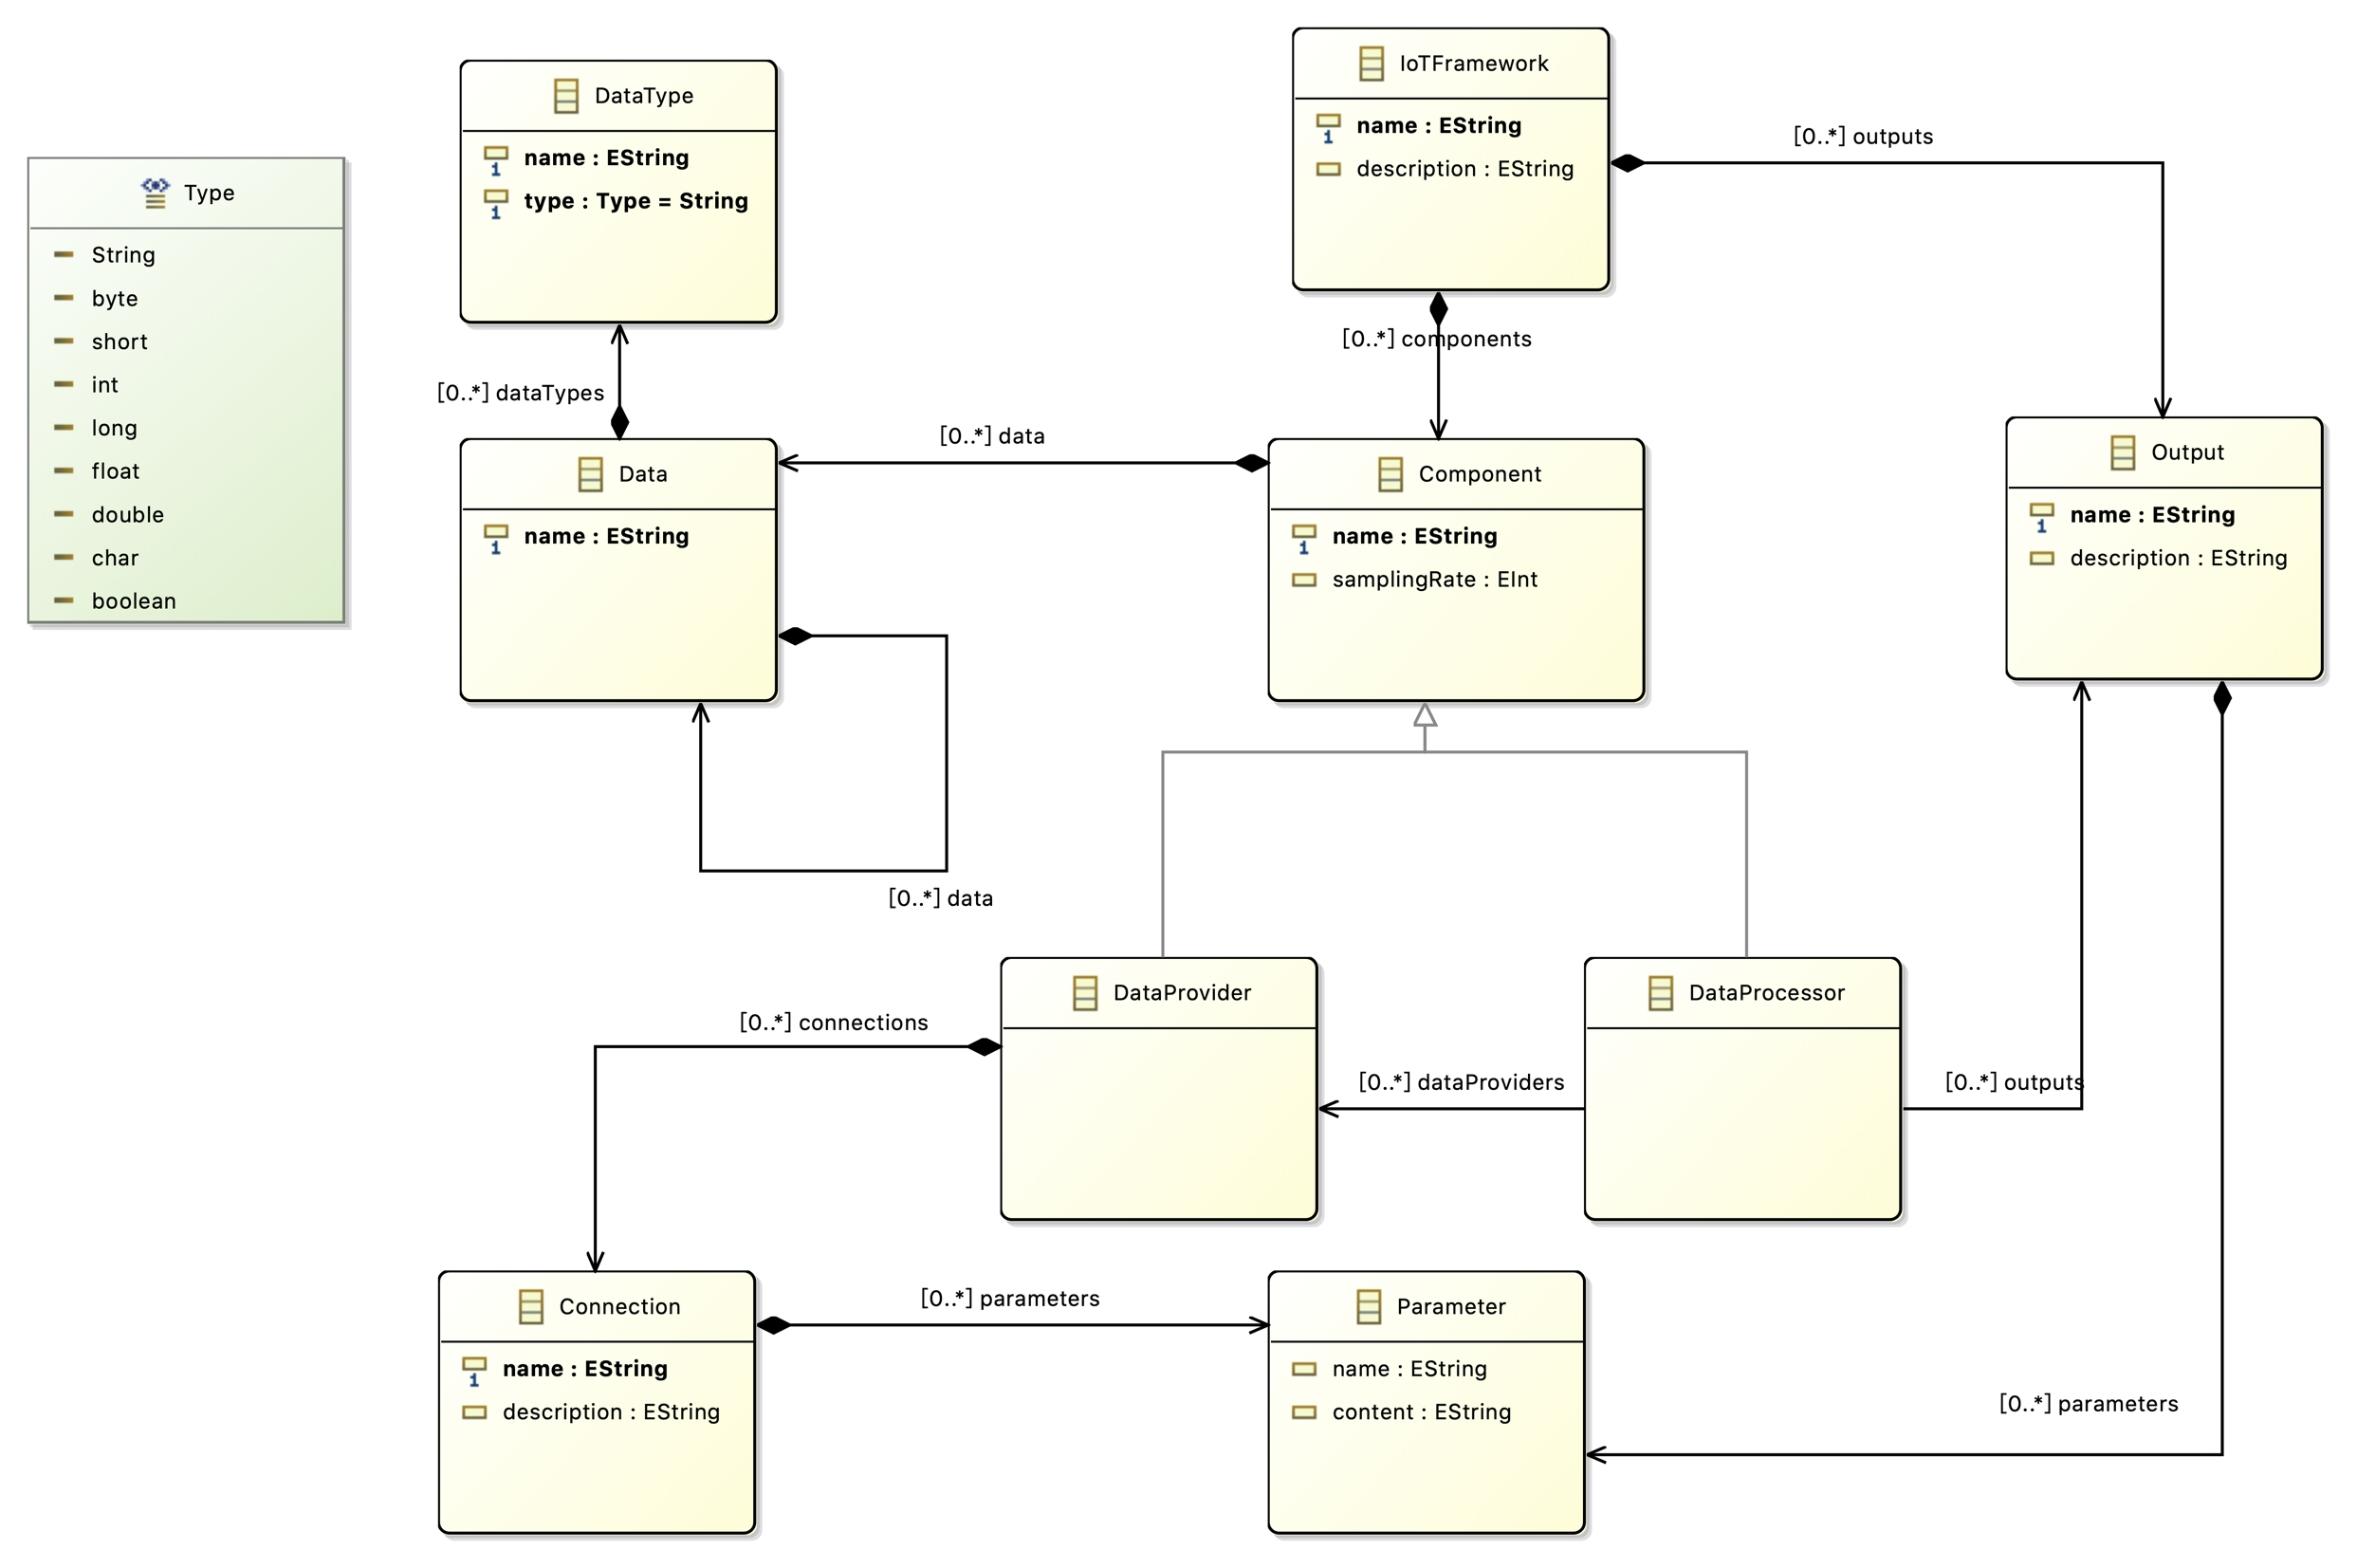
\includegraphics[width=0.9\textwidth]{iDSL class diagram.jpg} 
\caption{iDSL Ecore Class Diagram} 
\label{Fig.main1} 
\end{figure}

\subsection{Textual syntax}
\indent \par After the meta-model design is completed, we can create models that conform to it. But this needs to be done in EMF (Eclipse Modeling Framework) which can be a bit complicated for domain experts who don't familiar with Java. In order to make the entire modeling process easier and faster, we propose a new DSL called iDSL.\\
\indent \par In order to let domain experts get started faster, we try to make iDSL like XML. A tag is a markup construct that begins with "\textless" and ends with '\textgreater', which indicates a class or an attribute in the Meta-model. An element is a logical document component that begins with a start-tag and ends with a matching end-tag. The characters between the start-tag and end-tag, are the element's content, and may contain markup, including other elements, which are called child elements. Tag and content meet the rules of key-value pairs. An example is shown as followed:\par 
\indent \par
\textless Connection\textgreater \par
			\indent \indent bluetooth-ecg \par
			\indent \indent \textless description\textgreater'ecg-bluetooth-connection'\textless/description\textgreater \par
			\indent \indent \textless parameter\textgreater MAC\textless content\textgreater'AA:12:34:AA:12:34'\textless/content \textgreater \textless/parameter\textgreater \par
\textless/Connection \textgreater \par
\indent \par By doing so, domain experts can do their modeling work at ease without difficulties in terms of the syntax. See Appendix A for the complete textual model in iDSL.


\subsection{Model example}
\indent \par A graphic model example of ECG and EEG signals synchronization that conforms to the meta-model with Sirius tool\cite{ref20} is shown below in Fig.2 . 
\begin{itemize}
\item ECG/EEG device are two data providers according to the meta-model, both of them have certain data structure and connection types.
\item ecg/eeg SignalWindow corresponds to the data structure of the two signals respectively. Both have attributes of duration and period and sub structure of ecg/eeg Signal. Here they are similar, but may not be in other cases.
\item ecg/eeg Signal represents the signal structure collected and transmitted by IoT devices. It should be pointed out that although both of them contain time-stamps and values, they are different in data types, such as the value type may be integer or float or other types.
\item Synchroniser is where we preprocess the signals, that is, the synchronization operation. It receives signals from both devices, performs synchronization, and outputs as required. 
\item BT means Bluetooth connection, it may contain information of UUID, MAC address, etc. 
 \item db and monitor represent the output types, db is the abbreviation of database,  if output type is database, it will contain parameters like hostname, port, db name, etc. Monitor means output the results directly to the screen. 
\end{itemize}


\begin{figure}[htbp] 
\centering 
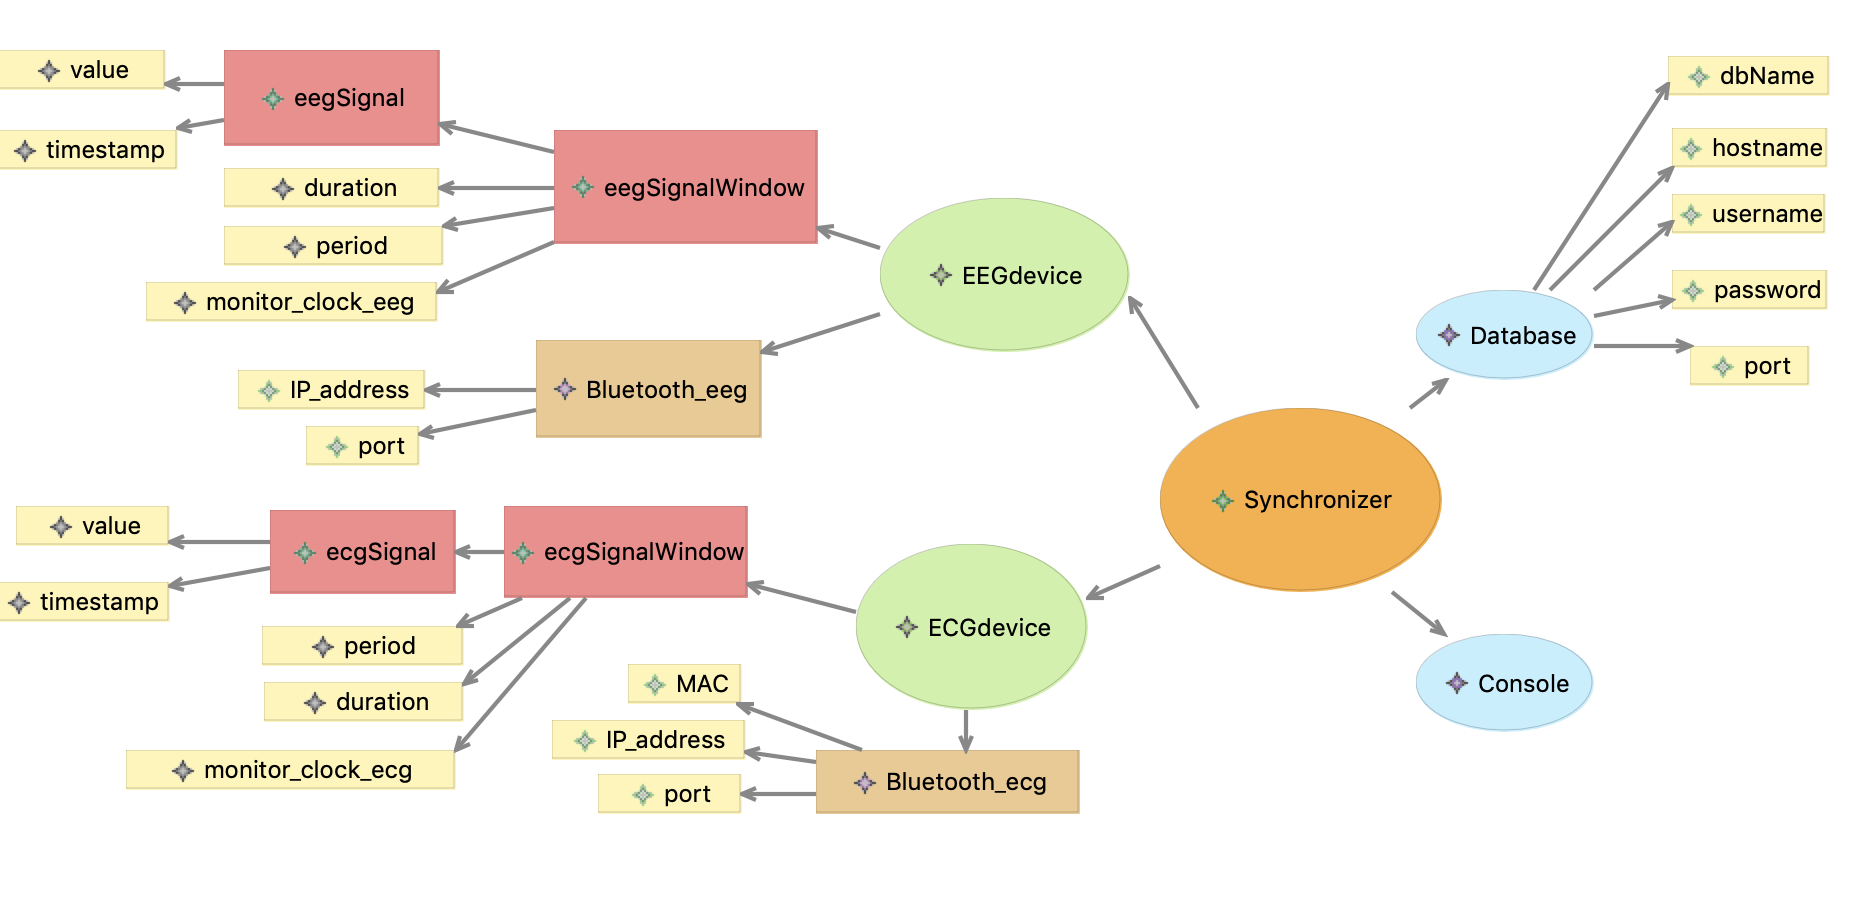
\includegraphics[width=0.9\textwidth]{Sirius-iDSL.png} 
\caption{A model example of ECG and EEG signals synchronization} 
\label{Fig.main2} 
\end{figure}


\section {Verification Issues}
\indent \par Here we study how solution providers are ensuring that their applications are fit for purpose. This includes, amongst other considerations, ensuring they are scalable, and interoperable.

\indent \par In order to ensure that the created model meets the requirements, we can add some constraints at the meta-model level or the model level. Some OCL examples are as follows:
\begin{itemize}
\item There must be at least one input (DataProvider).
\item Input must contain at least one sampling rate and one connection type, sampling rate must be positive. 
\item Connection parameters must conform to certain rules, like MAC or IP address.
\item There must be at least one output.
\item The parameters necessary for different output types. e.g., if output type is database, it must have hostname, port, db name, username, password, etc.
\end{itemize}


\section {Existing IoT Platforms and applications}
\indent \par In the field of Model-Driven Engineering, there are already some platforms and applications developed for the Internet of Things.
\begin{itemize}
\item MARTE (Modeling and Analysis of Real-Time and Embedded systems)\cite{ref5} provides support for specification, design, and verification/validation stages. These are then refined for both modeling and analyzing concerns. Modeling parts provides support required from specification to detailed design of real-time and embedded characteristics of systems. Analyzing parts provide facilities to annotate models with information required to perform specific analysis, especially, on performance and schedulability analysis.
\item openHAB\cite{ref9} represents a general-purpose framework for smart home gateways and is fully based on the Eclipse SmartHome project, which allows building smart home solutions as the most common application area of IoT. The heterogeneity and connectivity are supported by OSGi plug-ins called bindings and APIs in the OpenHAB framework.
\item ThingML (Internet of Things Modeling Language)\cite{ref18}  is an MDE approach that aims to cover a considerable amount of IoT use cases. The main contribution of the project is a code generation framework and an associated methodology to give practitioners full control of the code by letting them easily customize compilers for their needs. To accomplish this, expertise in MDE and Domain Specific Language (DSL) is required.
\end{itemize}



\section{Transformation}
\indent \par The goal of transformation in this project is to automatically generate executable code and rigorously check needed properties. To do so, we  need to ensure the transformation from the model into both Java and formal language LOTOS respectively. To do so, we use the Acceleo\cite{ref21} utility from the Obeo company. Through  these transformations, experts in different domains can perform different operations on models that conform to the meta-model from their own research perspectives. 


\subsection{To Java}
\indent \par We first focus on the transformation from model to Java code. According to the meta-model, we use the Acceleo tool to write conversion code to realize the transformation from model to text (M2T), and automatically generate the whole framework of a project model, including all classes and attributes as well as getters/setters for all attributes. What needs to be pointed out is, from the model, one can only get the main framework of the Java project, including the definition of classes and attributes, however, methods need to be added later.\\
\indent \par According to the model in Fig. 2, the corresponding UML class diagram is shown in Fig. 3. See Appendix B for the Acceleo code. \\
\indent \par As for our concrete study case, after the transformation, we can add the methods responsible for connecting IoT devices and the signal synchronization method to the framework. 


\begin{figure}[htbp] 
\centering 
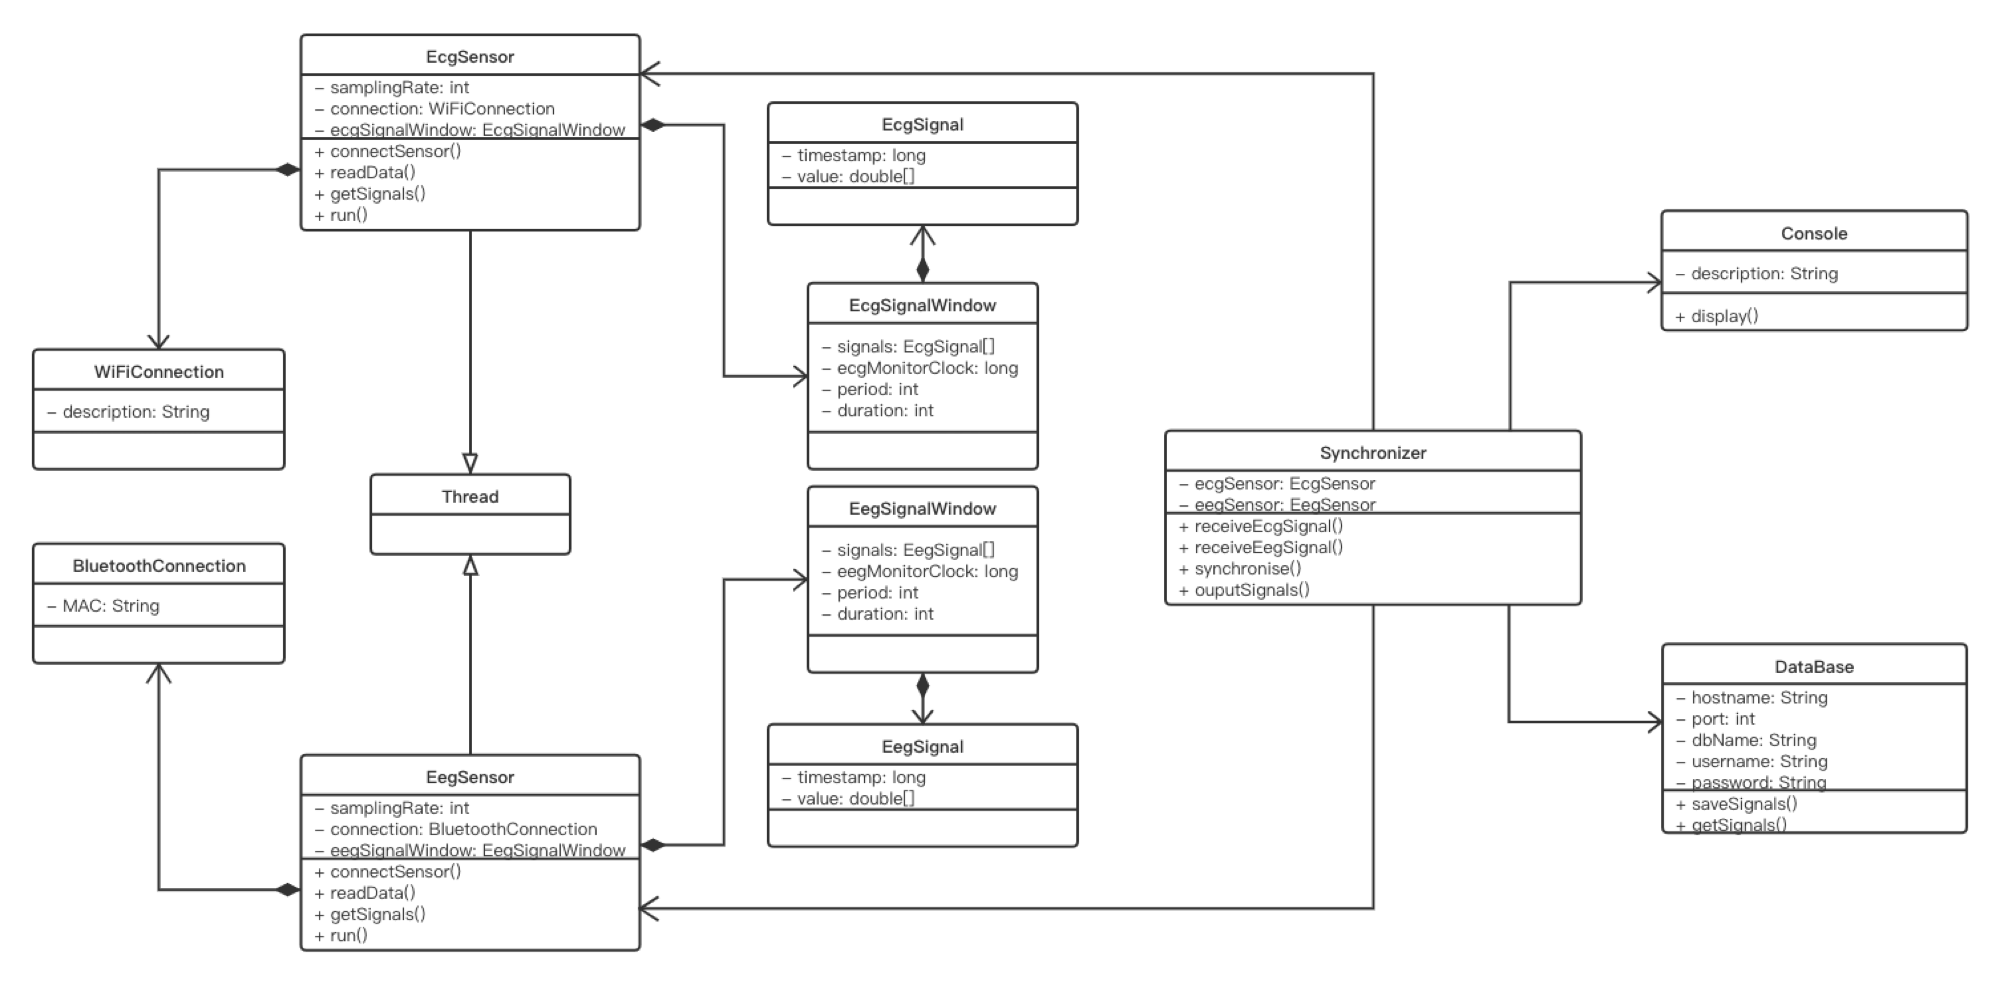
\includegraphics[width=0.9\textwidth]{UML-model.png} 
\caption{UML class diagram of the model} 
\label{Fig.main3} 
\end{figure}

\subsection{Signal synchronization}
\indent \par After getting the automatically generated framework, we can continue to work on the signal synchronization. It mainly contains 3 parts: 1) Connect to the IoT devices, here it means both ECG device and EEG device. 2) Extract signals' time-stamp and perform synchronization operation, 3) Output the synchronized signals according to the model. 

\subsubsection{Connect to devices}
\indent \par One of the heterogeneities of the Internet of Things is the diversity of device connection methods. Popular methods include Bluetooth, ZigBee, WiFi, Lora, NB-IoT, etc. \\
\indent \par In our simulated scenario, we assume that the connection has been established and we use Socket with C/S mode to exchange data. The monitor acts as server to keep listening the connection request from clients. Both ECG and EEG devices act as client, once connected to the monitor, they will send out signals which contain local clock (time-stamps) and data collected from sensors. \\
\indent \par The IoT devices may have different local clock, in order to achieve signal synchronization, our approach is to record the current monitor local time when the monitor receives a signal's first data, and use it as a reference to calibrate the local clock of the IoT devices.

\subsubsection{Synchronization operation}
\indent \par In our study case, the so-called ECG and EEG signals are different in nature, meaning that the ECG signal is continuous while the EEG one is event-driven and so discontinuous. This reflected in the synchronization operation means the monitor performs the synchronization only when it receives signals from both devices in the same time. \\
\indent \par To do so, we need parameters include: local time clock, sampling rate and monitor recorded clock of both continuous and discontinuous signal. And we define an offset as a monitor recorded clock minus a local time clock. What we need to find is the local time-stamp of the continuous signal that actually corresponds to the discontinuous signal's local clock, we call it "head" here. It is worth noting that when we try to find the "head" by using the two offsets, the result may not correspond to any sample in the continuous signals due to the sampling rate, under such circumstance, we try to find the closest time-stamp in the continuous signals. The detailed codes with comments and full Javadoc can be found in \cite{ref22}.

\subsubsection{Output operation}
\indent \par The ways of output have been indicated in the modeling stage. It needs to be implemented in the output operation. A possible example is that the model indicates to output to a certain database, then in the output operation, we need to use the information provided by the model to connect to the very database first, and then store the synchronized signals in it. This operation needs to be executed every time there is new synchronized data. 


\subsection{To LOTOS}
\indent \par  By using LOTOS\cite{ref19}, we can verify the needed properties base on the model we create. As before, the Acceleo tools can also be used to achieve the transformation. Each data provider or data processor in the model represents a "noexit" process in LOTOS and runs in parallel. All data providers communicate with data processors to send out data they collected, but they do not interact with each other. \\
\indent \par A possible example is to verify if the synchronization operation only occurs when it receives both the two inputs in the same time. For this signal synchronization system, the events include Input, Synchronize and Output. These events are all parallel. Inputs will transmit data to Synchronize, and Synchronize only happens when there are two inputs at the same time. Synchronize will then transmit synchronized data to Output. There is no directly data exchange between Input and Output. 




\section{Conclusion and future work}
\indent \par In this project, we proposed a new DSL called iDSL for IoT based on MDE. We first start by defining a meta-model with high generality, then create model instances and write OCL restrictions, and then create a XML-like textual syntax we called iDSL so that users can easily define their desired meta-model models through text. After the model has been defined, the model-to-text transformation can be realized automatically by using the M2T plugin we created to convert the model into executable Java code, and then simulation experiment has been performed, including simulation of ECG and EEG device connection, data transmission, synchronization operation and output execution.\\
\indent \par It is then proved to be helpful in concrete case in the healthcare field, which mainly focus on the signals synchronization between both EEG and ECG devices. The needed codes for different domains can be generated automatically, such as Java code or LOTOS script. By doing so, the advantages of Model-Driven Engineering including reusability and verifiability are shown.\\
\indent \par The Internet of Things has a variety of applications. In our case, we focus on the medical and healthcare field, that is, the synchronization of ECG and EEG signal. Therefore, in the modeling process, we only have data providers and data processors, but no actuators. However, the role of actuators is very important in some applications. This is a missing part of our current meta-model, which should be filled in in future work.\\
\indent \par Another future work is the implementation of formal verification with LOTOS in different perspectives. 


\section*{Acknowledgements}
\indent \par This research was partially supported by IRIT, Toulouse, France. We thank Meriem Ouederni and Lotfi Chaari for their judicious comments and the fruitful discussions throughout the research. 


\begin{thebibliography}{99}  
\bibitem{ref1}H. Al-Hamadi, A. Gawanmeh and M. Al-Qutayri, "Formalizing electrocardiogram (ECG) signal behavior in event-B", 2014 IEEE 16th International Conference on e-Health Networking, Applications and Services (Healthcom), 2014, pp. 55-60, doi: 10.1109/HealthCom.2014.7001813.  
\bibitem{ref2}Machado, Sergio et al, "Changes in Cortical Activity During Real and Imagined Movements: an ERP Study", Clinical practice and epidemiology in mental health : CP and EMH vol. 9 196-201. 15 Nov. 2013, doi:10.2174/1745017901309010196. 
\bibitem{ref3}Huang G., Meng J., Zhang D., Zhu X, "Window Function for EEG Power Density Estimation and Its Application in SSVEP Based BCIs", In: Jeschke S., Liu H., Schilberg D. (eds) Intelligent Robotics and Applications. ICIRA 2011. Lecture Notes in Computer Science, vol 7102. Springer, Berlin, Heidelberg, doi:10.1007/978364225489514. 
\bibitem{ref4}Covantes-Osuna C., Paredes O., Vélez-Pérez H., Romo-Vázquez R, "Window Functions Analysis in Filters for EEG Movement Intention Signals", In: González Díaz C. et al. (eds) VIII Latin American Conference on Biomedical Engineering and XLII National Conference on Biomedical Engineering. CLAIB 2019. IFMBE Proceedings, vol 75. Springer, Cham, doi:10.1007/978-3-030-30648-925.
\bibitem{ref5}Ciccozzi F., Spalazzese R, "MDE4IoT: Supporting the Internet of Things with Model-Driven Engineering", In: Badica C. et al. (eds) Intelligent Distributed Computing X. IDC 2016. Studies in Computational Intelligence, vol 678. Springer, Cham, doi:10.1007/978-3-319-48829-57.
\bibitem{ref6}Süß, Jörn Guy, Pop A, Fritzson P, et al. "Towards integrated model-driven testing of scada systems using the eclipse modeling framework and modelica", 19th Australian Conference on Software Engineering (aswec 2008). IEEE, 2008.
\bibitem{ref7}Abdoulaye Gamatié, Thierry Gautier, "The Signal Synchronous Multiclock Approach to the Design of Distributed Embedded System", IEEE Transactions on Parallel and Distributed Systems, Institute of Electrical and Electronics Engineers, 2010, 21 (5), pp.641-657. 10.1109/TPDS.2009.125. hal-00550056.
\bibitem{ref8}Alur, Rajeev. "Formal Verification of Hybrid Systems". Proceedings of the Ninth ACM International Conference on Embedded Software (2011): 273-78. Web.
\bibitem{ref9}Salihbegovic A, Eterovic T, Kaljic E, et al. "Design of a domain specific language and IDE for Internet of things applications", 2015 38th International Convention on Information and Communication Technology, Electronics and Microelectronics (MIPRO). IEEE, 2015: 996-1001.
\bibitem{ref10}A. Filieri et al., "Software Engineering Meets Control Theory", 2015 IEEE/ACM 10th International Symposium on Software Engineering for Adaptive and Self-Managing Systems, 2015, pp. 71-82, doi: 10.1109/SEAMS.2015.12.
\bibitem{ref11}B. Ramachandran and S. Bashyam, "Development of real-time ECG signal monitoring system for telemedicine application", 2017 Third International Conference on Biosignals, Images and Instrumentation (ICBSII), 2017, pp. 1-4, doi: 10.1109/ICBSII.2017.8082285.
\bibitem{ref12}Khan M.S., Sikder R., Adnan M.A., "A Hybrid Approach for Synchronizing Clocks in Distributed Systems", In: Da Silva D., Wang Q., Zhang LJ. (eds) Cloud Computing – CLOUD 2019. CLOUD 2019. Lecture Notes in Computer Science, vol 11513. Springer, Cham, doi:10.1007/978303023502419.
\bibitem{ref13}Ahmad S, Malik S, Ullah I, Park D-H, Kim K, Kim D. "Towards the Design of a Formal Verification and Evaluation Tool of Real-Time Tasks Scheduling of IoT Applications". Sustainability. 2019; 11(1):204, doi:10.3390/su11010204
\bibitem{ref14}Pramudianto, Ferry, Indra Rusmita Indra, and Matthias Jarke. "Model Driven Development for Internet of Things Application Prototyping". SEKE. 2013.
\bibitem{ref15}Nepomuceno, Thiago, et al. "AutoIoT: a framework based on user-driven MDE for generating IoT applications". Proceedings of the 35th Annual ACM Symposium on Applied Computing. 2020.
\bibitem{ref16}Rouse, Margaret (2019). "internet of things (IoT)". IOT Agenda. Retrieved 14 August 2019.
\bibitem{ref17}Laplante, Phillip A.; Kassab, Mohamad; Laplante, Nancy L.; Voas, Jeffrey M. "Building Caring Healthcare Systems in the Internet of Things". IEEE Systems Journal. 12 (3): 3030–3037. Bibcode:2018ISysJ..12.3030L. doi:10.1109/JSYST.2017.2662602
\bibitem{ref18}Harrand N, Fleurey F, Morin B, et al. "ThingML: a language and code generation framework for heterogeneous targets", Proceedings of the ACM/IEEE 19th International Conference on Model Driven Engineering Languages and Systems. 2016: 125-135.
\bibitem{ref19}Turner, K.J. "Incremental requirements specification with LOTOS". Requirements Eng 2, 132–151 (1997). https://doi.org/10.1007/BF02802772
\bibitem{ref20}https://www.eclipse.org/sirius/
\bibitem{ref21}https://www.acceleo.org
\bibitem{ref22}https://github.com/JulienFan/iDSL
\end{thebibliography}


\clearpage 
\begin{appendices}

\section{Textual model in iDSL}
\indent \par With the help of Xtext tool, we created a new domain specific language called iDSL for modeling the IoT systems. A model example defined in iDSL is shown in Fig. 4. 
\begin{figure}[htbp] 
\centering 
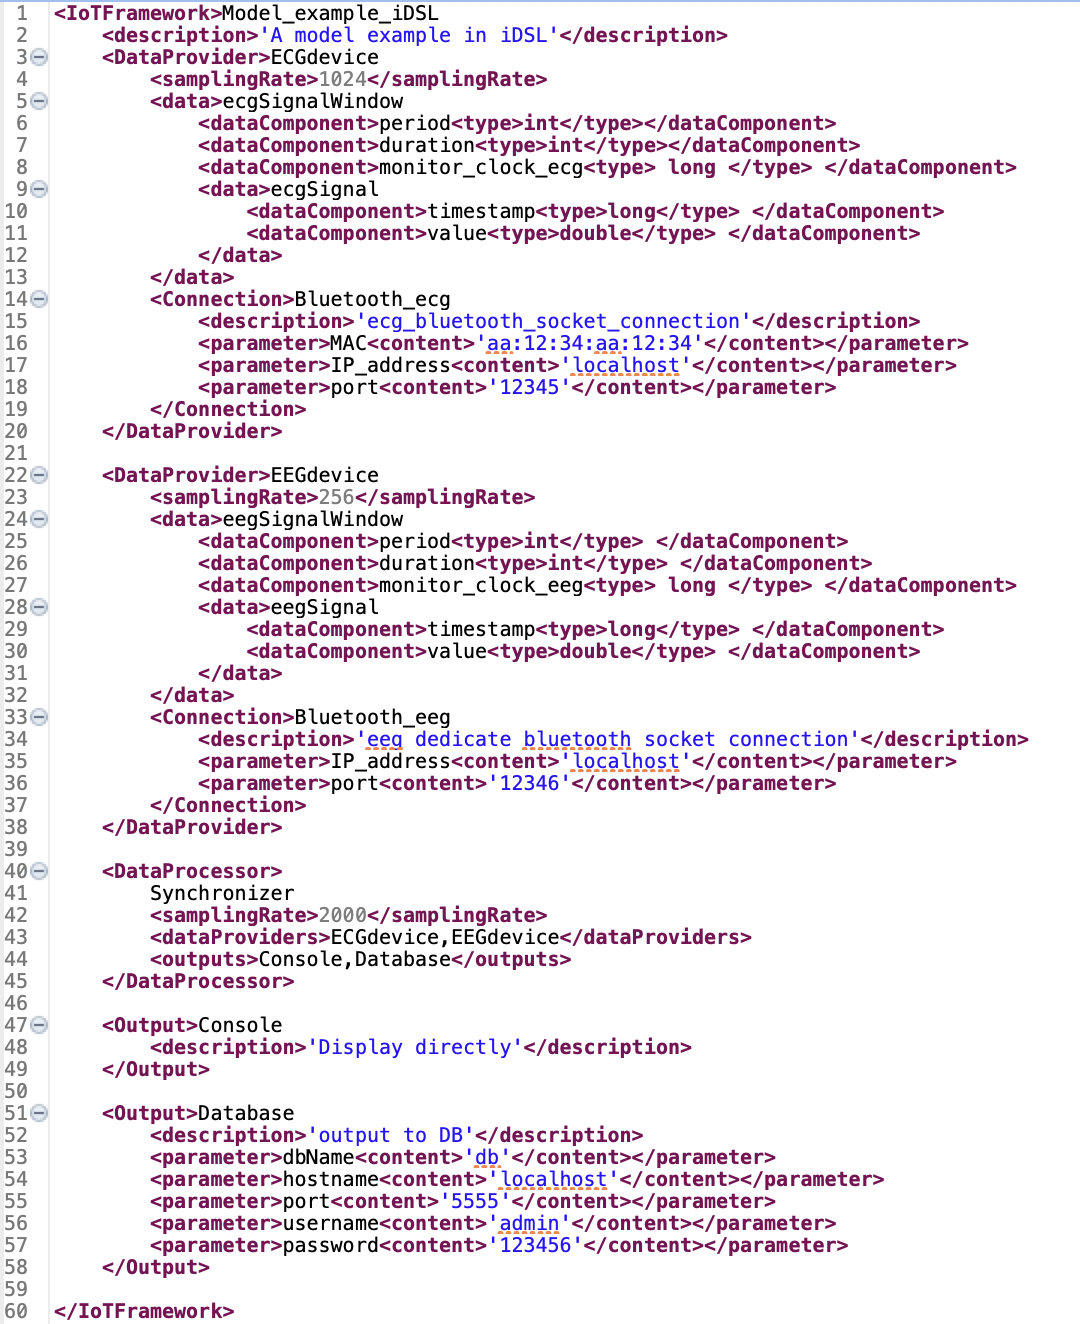
\includegraphics[width=0.6\textwidth]{Xtext-model.png} 
\caption{A model example defined in iDSL} 
\label{Fig.main4} 
\end{figure}

\clearpage
\section{Transformation from model to Java}
\indent \par By using Acceleo tool, we created a script that automatically converts the model into Java code. Including all classes and attributes as well as getters/setters for all attributes. The Acceleo script for model to Java transformation is shown in Fig. 5.

\begin{figure}[htbp]
\centering
\subfigure[Acceleo script 1]{
\label{Fig.sub.1}
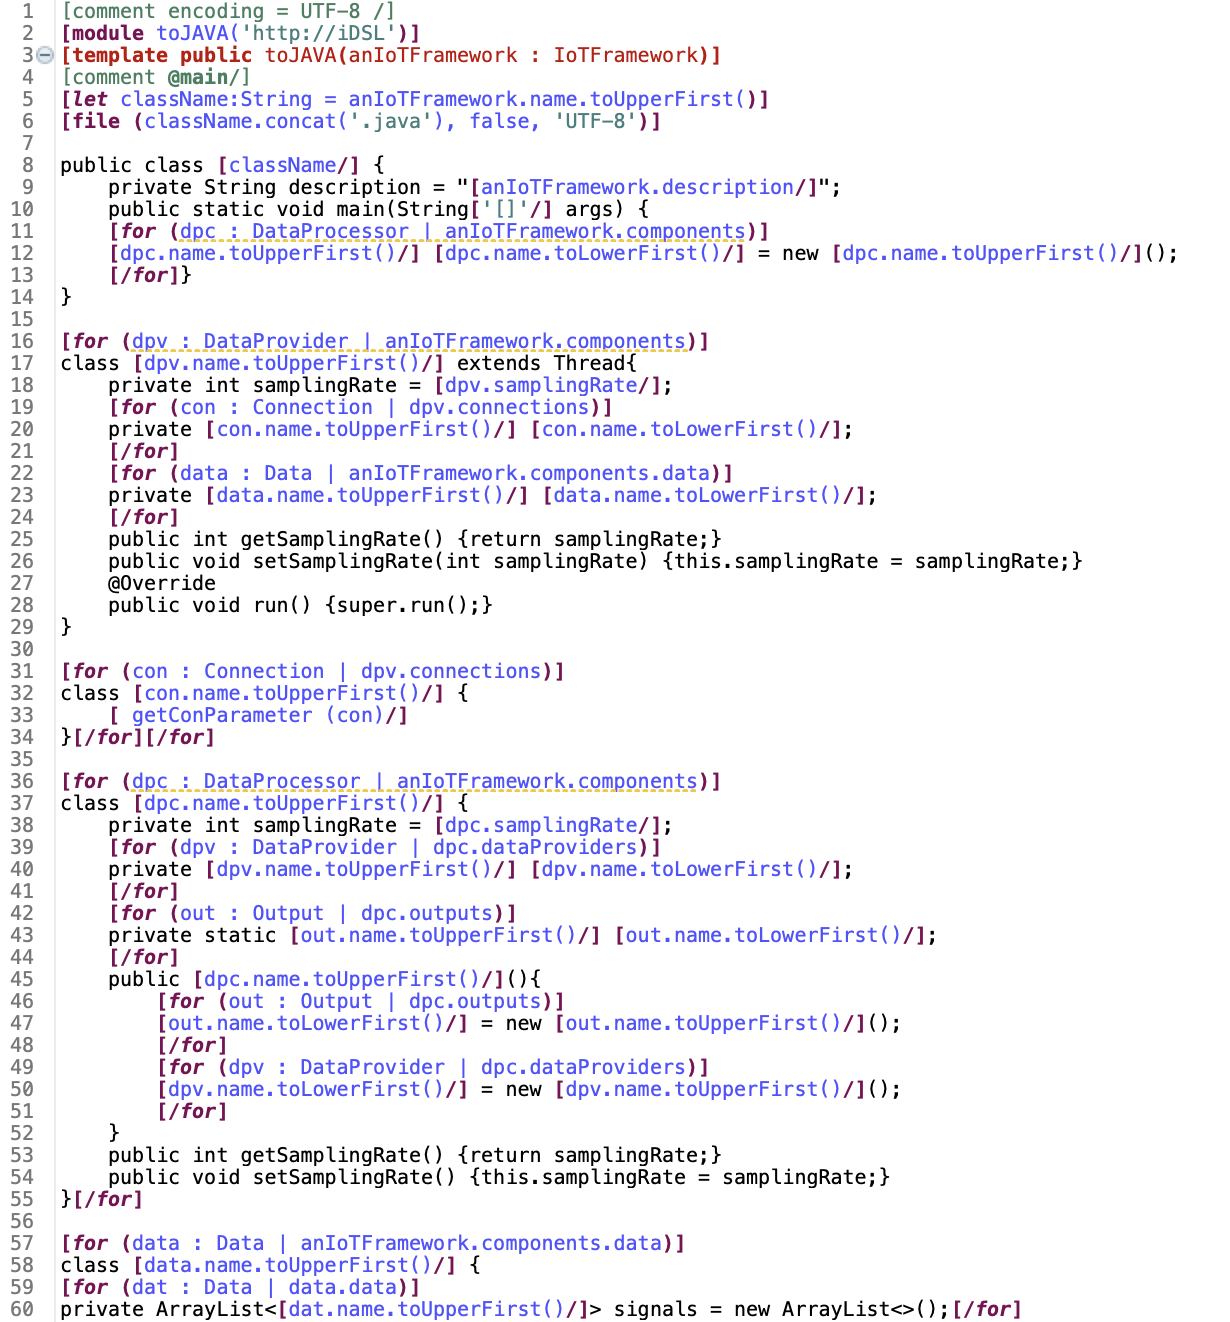
\includegraphics[width=0.48\textwidth]{Acceleo1.png}}
\subfigure[Acceleo script 2]{
\label{Fig.sub.2}
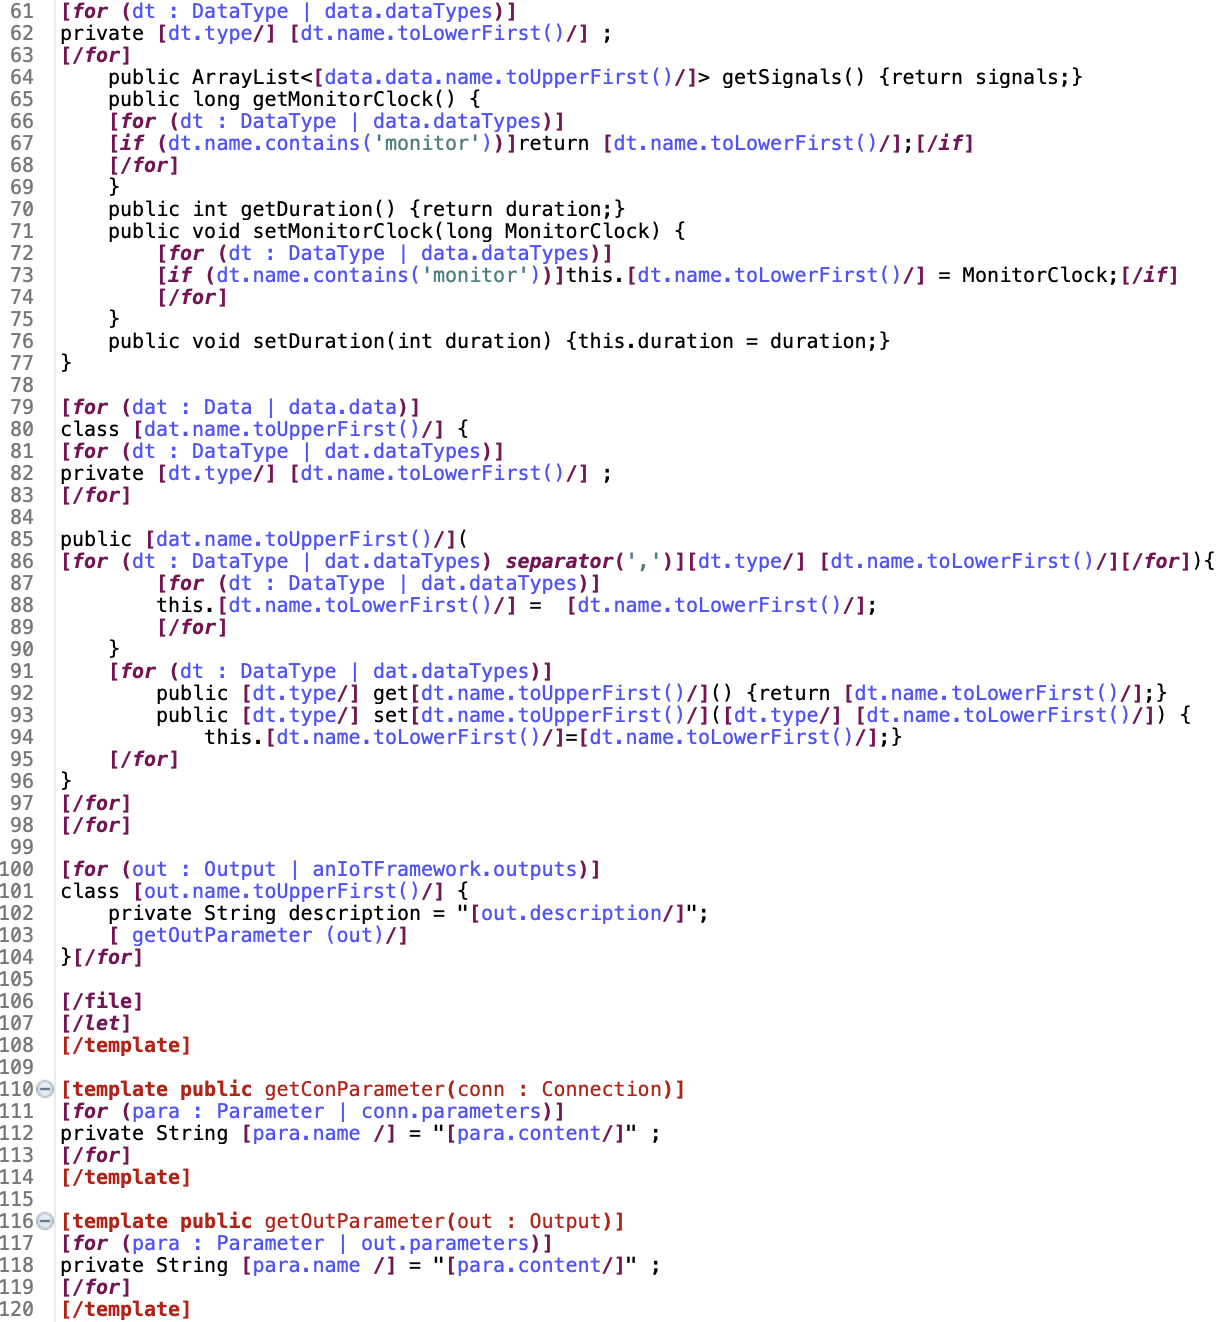
\includegraphics[width=0.48\textwidth]{Acceleo2.png}}
\caption{Model to Java transformation}
\label{Fig.lable}
\end{figure}


      
    
      
\end{appendices}





\end{document}  